\documentclass{article}
\usepackage{graphicx}
\usepackage[absolute,overlay]{textpos}
\setlength{\parindent}{0pt}
\usepackage{geometry}
\geometry{top=1in, bottom=1in, right=1in, left=1in}
\usepackage{multicol}
\usepackage{multirow}
\pagenumbering{arabic}

\usepackage{listings}
\usepackage{xcolor}
\usepackage{biblatex}
\usepackage{hyperref}
\usepackage{float}
\usepackage{array}
\usepackage{longtable}
\pagenumbering{arabic}

\usepackage{listings}
\usepackage{color}

\definecolor{dkgreen}{rgb}{0,0.6,0}
\definecolor{gray}{rgb}{0.5,0.5,0.5}
\definecolor{mauve}{rgb}{0.58,0,0.82}


\begin{document}
    \BgThispage
    \begin{titlepage}
    \centering
    \vspace*{200px}
    {\scshape\Huge \textbf{FRACSMART} \par}
    \vspace{3cm}
    {\itshape\Large  MEMORIA DESCRIPTIVA DEL PROGRAMA DE CÓMPUTO\par}
    \vfill
    {\Large Presenta: \par}
    {\Large \textbf{Montufar Benítez Marco Antonio} \par}
    \vspace{1cm}
    {\Large Versión: \par}
    {\Large \textbf{1.0}\par}
    \vfill
    {\Large Mayo 2026 \par}
    \end{titlepage}

%********************************************************

\newpage
\section*{Índice general}
\tableofcontents

%********************************************************

\newpage
\section{Índice de tablas}
\listoftables

%********************************************************

\newpage
\section{Índice de figuras}
\listoffigures

%********************************************************

\newpage
\section{Resumen}
\quad \quad 

%********************************************************

\newpage
\section{Introducción}
\quad\quad La gestión en un sector residencial exige el controlamiento de todos los residentes y sus viviendas. Recopilar, actualizar y archivar este tipo, de información de forma manual es complejo y tardado, de igual forma, implicaría realizar un seguimiento de múltiples procedimientos y preparar esos informes para las diferentes gestiones administrativas. \\

\quad\quad \textbf{\textit{FracSmart}}, versión 1.0, es un sistema diseñado para automatizar esos procesos, es una aplicación web desarrollada en \textit{R} utilizando la paquetería de \textit{Shiny}. Entre sus funciones principales, de esta versión inicial, se encuentran, buscar información sobre los residentes según su vivienda, rastrear sus marcas de garantía asociadas al desarrollo de la comunidad y actualizar las transacciones incluidas la fecha, el comprador, el marco, el importe, el método de pago, agente comercial, el tipo de marca de garantía y otros comentarios generales. Además \textbf{\textit{FracSmart}} muestra las transacciones en una tabla editable y genera informes en un formato de Microsoft Excel (.xlsx) con un resumen de las ventas categorizadas por la fecha y método de pago. \\

\quad\quad La memoria descriptiva que se presenta a continuación pretende describir en general las características funcionales y técnicas del programa informático \textbf{\textit{FracSmart}} para su inscripción en el Instituto Nacional del Derecho de Autor (INDAUTOR).

%********************************************************


\newpage
\section{Objetivo del sistema}
\quad\quad \textbf{\textit{FracSmart}} fue diseñado para proveer un método mas organizado de las ventas administrativas y operaciones que se llevan a cabo en una comunidad residencial. \\

\quad\quad El programa entiende una necesidad practica, con la información que refiere a los residentes y las propiedades que ya existen, pero que un operador administrativo puede necesitar para asociar esa información a nuevas transacciones de una forma mas consistente. Ya que realizar este proceso de forma manual requiere estar buscando constantemente la información del residente, su vivienda, domicilio entre otras cosas y después realizar el reporte correspondiente. \\

\quad\quad \textbf{\textit{FracSmart}} realiza estas actividades juntas en un solo entorno de trabajo.\\

\quad\quad En la versión 1.0, la aplicación esta principalmente orientada al registro de ventas de marbetes asociados con sus respectivos residentes y viviendas. Por cada transacción, el programa permite al operador registrar información como la fecha, cliente, calle, número de casa, cantidad total, método de pago, ID de marbete, tipo de marbete, ejecutivo de venta y notas adicionales.\\

\quad\quad El programa también asiste al operador con ciertas tareas repetitivas. Por ejemplo, puede buscar y localizar diversa información del residente desde un archivo de \textit{Excel} existente con solo la calle o numero de casa, calcular la cantidad de de la transacción según el número de marbetes, generar de forma dinámica el numero apropiado de campos para documentar la información del marbete y preparar un reporte de \textit{Excel} de las transacciones registradas durante la sesión. \\

\quad\quad El propósito general de la aplicación por lo tanto no es solo reproducir en una pantalla de computadora un formulario de papel. Su propósito es conectar varios procesos administrativos en un solo lugar.

%********************************************************


\newpage
\section{Descripción general}
\quad\quad \textbf{\textit{FracSmart}} es implementado como una aplicación web interactiva utilizando \textit{R} y \textit{Shiny}. \\

\quad\quad Cuando la aplicación es abierta, el operador es presentado con una pantalla principal identificada en la interfaz como: 

\begin{center}
    "Registro de Ventas - Solares" 
\end{center}

\quad\quad La pantalla principal es dividida en tres áreas funcionales
\begin{enumerate}
    \item Búsqueda del cliente e información del cliente.
    \item Información de la venta y detalle del marbete.
    \item Manejo de registros y acciones de salida.
\end{enumerate}

\quad\quad Una tabla de transacción se muestra abajo de estas áreas y enseña las ventas que se han registrado durante la sesión actual de la aplicación.\\

\quad\quad Esta configuración es eficaz en mantener el flujo del trabajo visible desde una sola pantalla. El operador puede localizar al residente, verificar o completar la información del cliente, meter la transacción, registrar el marbete correspondiente, y añadir la venta sin necesidad de estar buscando en diversas ventanas o aplicaciones individuales.\\

\quad\quad La interfaz es generada a través de \textit{Shiny} y por lo tanto es accesada por un navegador web. El programa corre en el procesador de \textit{R}.
%********************************************************


\newpage
\section{Alcance funcional}
\quad\quad La funcionalidad descrita en este documento corresponde especificamente al código fuente de \textbf{\textit{FracSmart}}, versión 1.0.\\

\quad\quad Las funciones principales son:
\begin{enumerate}
    \item Búsqueda de residente a través del domicilio.
    \item Recuperación automática de la información del residente a través de un libro de \textit{Excel}.
    \item Registro manual y modificación de la información del cliente.
    \item Entrada de la fecha de transacción.
    \item Selección del método de pago.
    \item Selección del número de marbetes.
    \item Cálculo automático del estándar de transacción.
    \item Entrada manual de la cantidad de ventas especiales.
    \item Generación dinámica de campos de identificación del marbete.
    \item Clasificación de cada marbete como "Normal" o "Tag".
    \item Selección del personal de venta.
    \item Entrada manual de otro personal de venta cuando sea requerido.
    \item Entrada adicional de notas de transacción.
    \item Adición de ventas nuevas a la tabla de transacción activa.
    \item Display de transacciones en una tabla iterativa.
    \item Selección y deselección de registros de transacción individuales.
    \item Generación de un reporte de \textit{Excel}.
    \item Generación de un resumen agrupado por fecha y método de pago.        
\end{enumerate}

\quad\quad El programa adicionalmente contiene una configuración de \textit{Gmail} al incluir un control de "Enviar por Email".

%********************************************************


\newpage
\section{Información manejada por el sistema}
\quad\quad \textbf{\textit{FracSmart}} maneja la información relacionada a tres áres principales, residentes, viviendas y transacciones.\\

\subsection{Información de residentes y viviendas}
\quad\quad La información del residente se obtiene de un libro de \textit{Excel} existente usado como fuente de referencia por la aplicación.\\

\quad\quad La información principal usada incluye:
\begin{itemize}
    \item Nombre del residente.
    \item Calle.
    \item Número de casa.
\end{itemize}

\quad\quad Esta información es usada para identificar la propiedad residencial asociada con la transacción.

\subsection{Información de transacción}
\quad\quad Por cada transacción, \textbf{\textit{FracSmart}} puede registrar:
\begin{itemize}
    \item Fecha.
    \item Nombre del cliente.
    \item Calle.
    \item Número de casa.
    \item Monto de transacción.
    \item Método de pago.
    \item Identificador de marbete.
    \item Tipo de marbete.
    \item Asesor de venta.
    \item Notas adicionales.
\end{itemize}

\quad\quad Estos campos proveen la información necesaria para identificar y revisar cada operación.

%********************************************************

\newpage
\section{Proceso general de operación}
\quad\quad La operación básica de \textbf{\textit{FracSmart}} puede ser resumida de la siguiente manera:

\begin{enumerate}
    \item El operador abre la aplicación a través de un navegador web.
    \item El residente o la propiedad relacionada a la transacción es identificada.
    \item \textbf{\textit{FracSmart}} consulta la información disponible y muestra los datos correspondientes.
    \item El operador registra la información de la transacción.
    \item El número e identificador de marbete es registrado.
    \item El método de pago y el asesor de la venta son seleccionados.
    \item Notas adicionales pueden ser ingresadas cuando sean necesarias.
    \item La transacción es añadida a los registros activos.
    \item Las transacciones registradas son mostradas en una tabla interactiva.
    \item Los registros incorrectos pueden ser removidos de ser necesario.
    \item Al termino del proceso, la información registrada se puede exportar a un Excel.
\end{enumerate}

\quad\quad Este flujo de trabajo permite las actividades administrativas principales asociadas con la venta sean registradas y completadas desde una misma aplicación.

%********************************************************

\newpage
\section{Estructura de software}
\quad\quad \textbf{\textit{FracSmart}} sigue la arquitectura de una aplicación web de \textit{Shiny}. \\

\quad\quad Su operación puede ser representada de forma simplificada como:
\begin{figure}[H]
        \centering
        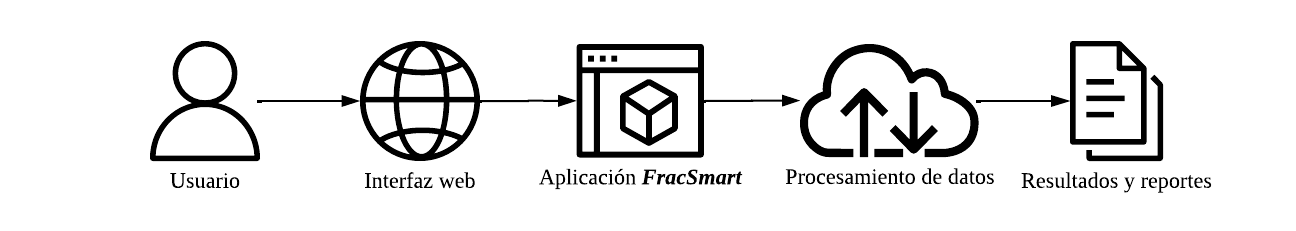
\includegraphics[width=1\linewidth]{imagenes/Entidad-Relación.png}
        \caption{Flujo de operaciones (Elaboración propia, 2026)}
        \label{fig:enter-label}
    \end{figure}

\subsection{Interfaz de usuario}
\quad\quad La interfaz de usuario es el componente visual por el cual el operador interactúa con \textbf{\textit{FracSmart}}. Incluye:

\begin{itemize}
    \item Campos de texto.
    \item Selección de menus.
    \item Controles de fecha.
    \item Botones.
    \item Formularios de transacción.
    \item Tablas.
    \item Controles de descarga.
\end{itemize}

\quad\quad La interfaz fue diseñada para organizar el proceso de las transacciones en secciones claras y para reducir la cantidad de información que debe ser manejada de forma manual.\\

\subsection{Lógica de la aplicación}
\quad\quad La lógica de la aplicación mesta implementada en \textit{R}. Es resposable por tareas como:
\begin{itemize}
    \item Leer la información del residente.
    \item Procesar los datos del residente.
    \item Crear registros de transacciones.
    \item Actualizar la tabla de transacción.
    \item Remover registros seleccionados.
    \item Organizar la información.
    \item Generar reportes de \textit{Excel}.
\end{itemize}

\quad\quad \textit{Shiny} conecta la interfaz gráfica con estas funciones y actualiza la información mostrada conforme el operador interactúa con el programa.

%********************************************************

\newpage
\section{Tecnología utilizada}
\quad\quad 

%********************************************************

\newpage
\section{Manejo de datos}
\quad\quad La versión 1.0 de FracSmartt utiliza Microsoft Excel como parte del proceso de manejo de datos.\\

\quad\quad La información del residente es obtenida de un libro externo llamado "solares.xlsx". Este archivo funciona como fuente de referencia que le permite a FracSmart asociar las direcciones con la información general del residente. \\

\quad\quad Las transacciones nuevas que son registradas durante la operación se manejan con una aplicación activa de Shiny.\\

\quad\quad La versión actual no utiliza un sistema de bases de datos como MySQL, SQLite, entre otros, para su almacenamiento transaccional.

%********************************************************

\newpage
\section{Reportes}
\quad\quad Uno de los principales datos de salida generados por FracSmart es un reporte de Microsoft Excel.\\

\quad\quad El reporte contiene las transacciones registradas durante la sesión trabajada, incluyendo información como el cliente, su propiedad, la cantidad, el método de pago, el asociado de venta, el marbete, y notas. \\

\quad\quadLas transacciones son agrupadas conforme la fecha y el método de pago. Para cada grupo el reporte provee el numero de ventas y el total correspondiente.\\

\quad\quad Esto permite que el reporte provee información detallada en cuanto a las transacciones individuales y un reporte mas conciso de la actividad registrada durante el periodo.

%********************************************************

\newpage
\section{Plataforma y entorno de ejecución}
\quad\quad FracSmart esta diseñada para ser una aplicación basada en el navegador. \\

\quad\quad La interfaz gráfica es mostrada a través de un navegador web, mientras que la aplicación en si opera en un entorno capaz de correr R y Shiny. \\

\quad\quadPorque el programa utiliza una interfaz web, puede ser mostrado en diferentes dispositivos capaz de utilizar navegadores, cuando la aplicación de Shiny esta propiamente alojada o disponible a través del entorno correspondiente.\\

\quad\quad El software requiere las librerías de R, y archivos secundarios que esten disponibles para la ejecución del entorno y asi todas las funciones se ejecuten de forma correcta.

%********************************************************

\newpage
\section{Resumen técnico}
\quad\quad 

%********************************************************

\newpage
\section{Referencias bibliográficas}

    \begin{thebibliography}{99}
        \bibitem{mcmillan2008}
        McMillan, J. H. y Schumacher, S. (2008). \textbf{\textit{Investigación educativa: Una introducción conceptual}} (5ª ed.). Pearson Educación.
    
    \end{thebibliography}

\end{document}
